%-------------------------
%makefile
%(c) H.Buchmann FHNW 2014
%export TEXINPUTS=${HOME}/fhnw/edu/:${HOME}/fhnw/edu/tinL/config/latex:${HOME}/fhnw/edu/config//:
%-------------------------
\documentclass{beamer}
\usepackage{latex/beamer}
%---------------------
%local defines
%(c) H.Buchmann FHNW 2009
%$Id$
%---------------------
\newcommand{\target} {\beaglebone\xspace}
\newcommand{\targetS}{{\bf BBG}\xspace}
\newcommand{\host}   {{\em Host}\xspace}
\newcommand{\targetroot} {{\bf target-root}\xspace}
\newcommand{\kernel} {{\bf kernel}\xspace}
\renewcommand{\c}{{\bf C}\xspace}
\newcommand{\cpp}{{\bf C++}\xspace}
\newcommand{\posix}{{\bf POSIX}\xspace}

\input{/home/buchmann/latex/dirtree/dirtree.tex}

\usepackage[absolute]{textpos}
\setlength{\TPHorizModule}{1mm}
\setlength{\TPVertModule}{1mm}

\begin{document}

\newcommand{\uboot}{{U-Boot \xspace}}

\title[Assembly]{Zusammenbau\\Assembly}

\frame{\titlepage}

\begin{frame}{Um was geht es ?}{Ein erstes vollst�ndiges System}
 \begin{itemize}
  \item Bootloader \uboot
  \item \kernel
  \item \unix 
 \end{itemize}
\end{frame}

\begin{frame}{Die Schichten}
\begin{center}
 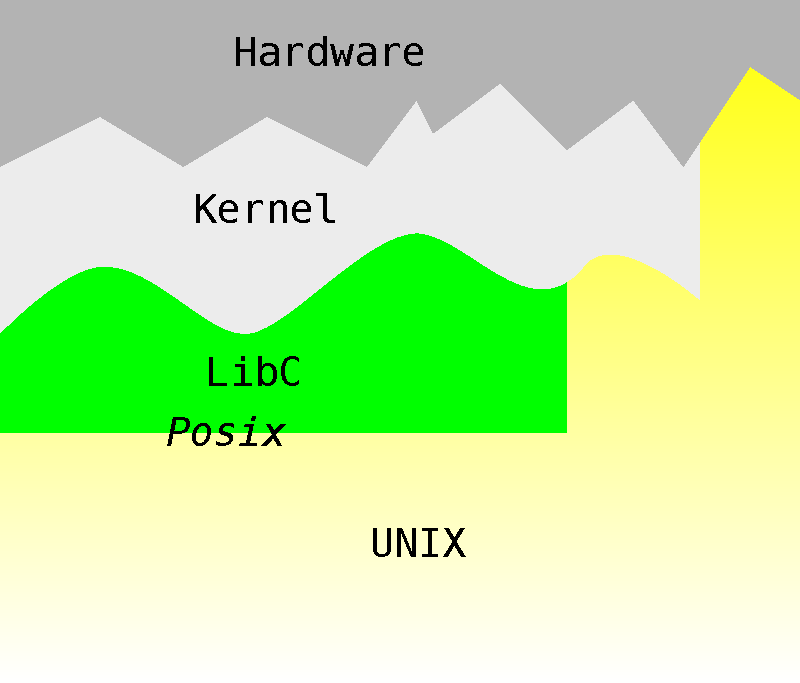
\includegraphics[width=0.75\textwidth]{../../5-kernel/doc/layers.pdf}
\end{center}
\end{frame}

\begin{frame}{Das Ziel}{f�r \targetS}
 \begin{block}{Nach dem Reset:}
 \begin{enumerate}
  \item \uboot startet \kernel
  \item \kernel startes \unix
  \item \unix 
   \begin{itemize}
    \item konfiguriert {\em ethernet �ber USB}
    \item startet \cod{ssh} Server 
   \end{itemize}
 \end{enumerate}
 \end{block}
\end{frame}

\begin{frame}{Was wir schon haben}
 \begin{description}[root Filesystem:]
  \item[Toolchain:] download
  \item[\uboot:] selber gemacht
  \item [\kernel:] selber gemacht
  \item[root Filesystem:] download
  \begin{itemize}
   \item libc/\unix
  \end{itemize} 
 \end{description}
\end{frame}

\begin{frame}{Die Partitionen und Filesysteme}
 \begin{description}
  \item[p1] bootfs:vfat $\approx 20MiB$
   \begin{itemize}
    \item \uboot
    \begin{itemize}
     \item \cod{MLO}  
     \item \cod{u-boot.img}
     \item \cod{uEnv.txt} Konfiguration
    \end{itemize}
    \item \kernel
    \begin{itemize}
      \item \cod{zImage}
	  \item \cod{am335x-boneblack-wireless.dtb}
    \end{itemize}
   \end{itemize}
  \item[p2] rootfs:ext4 $\approx 200MiB$
  \begin{itemize}
   \item \cod{etc/init.d/rcS} init-script
  \end{itemize}
 \end{description}
\end{frame}

\section{\uboot}
\begin{frame}{\uboot}{Wichtige Befehle}
 \begin{itemize}
  \item \cod{boot} startet \cod{bootcmd}
  \item \cod{fatload mmc 0 {\em addr} {\em file}}
  \item \cod{setenv {\em key} {\em value}}
  \item \cod{run {\em script}}
  
  \remark{Siehe \url[http]{www.denx.de/wiki/view/DULG/UBootCmdGroupEnvironment}}
 \end{itemize}
\end{frame}

\begin{frame}{\uboot}{Wichtige Variablen}
\begin{itemize}
 \item \cod{bootcmd} f�r \uboot \cod{boot}
 \item \cod{bootargs} f�r den \kernel
\end{itemize}
\end{frame}

\begin{frame}{\uboot}{Wichtiger File}
 \begin{itemize}
  \item \cod{uEnv.txt} setzt:
  \begin{itemize}
   \item \cod{bootcmd}
   \item load-script f�r den\kernel
   \item \cod{bootargs}
  \end{itemize}
 \end{itemize}
\end{frame}

\section{Kernel}

\begin{frame}{Konfiguration}{USB-Gadget Support}
\begin{center}
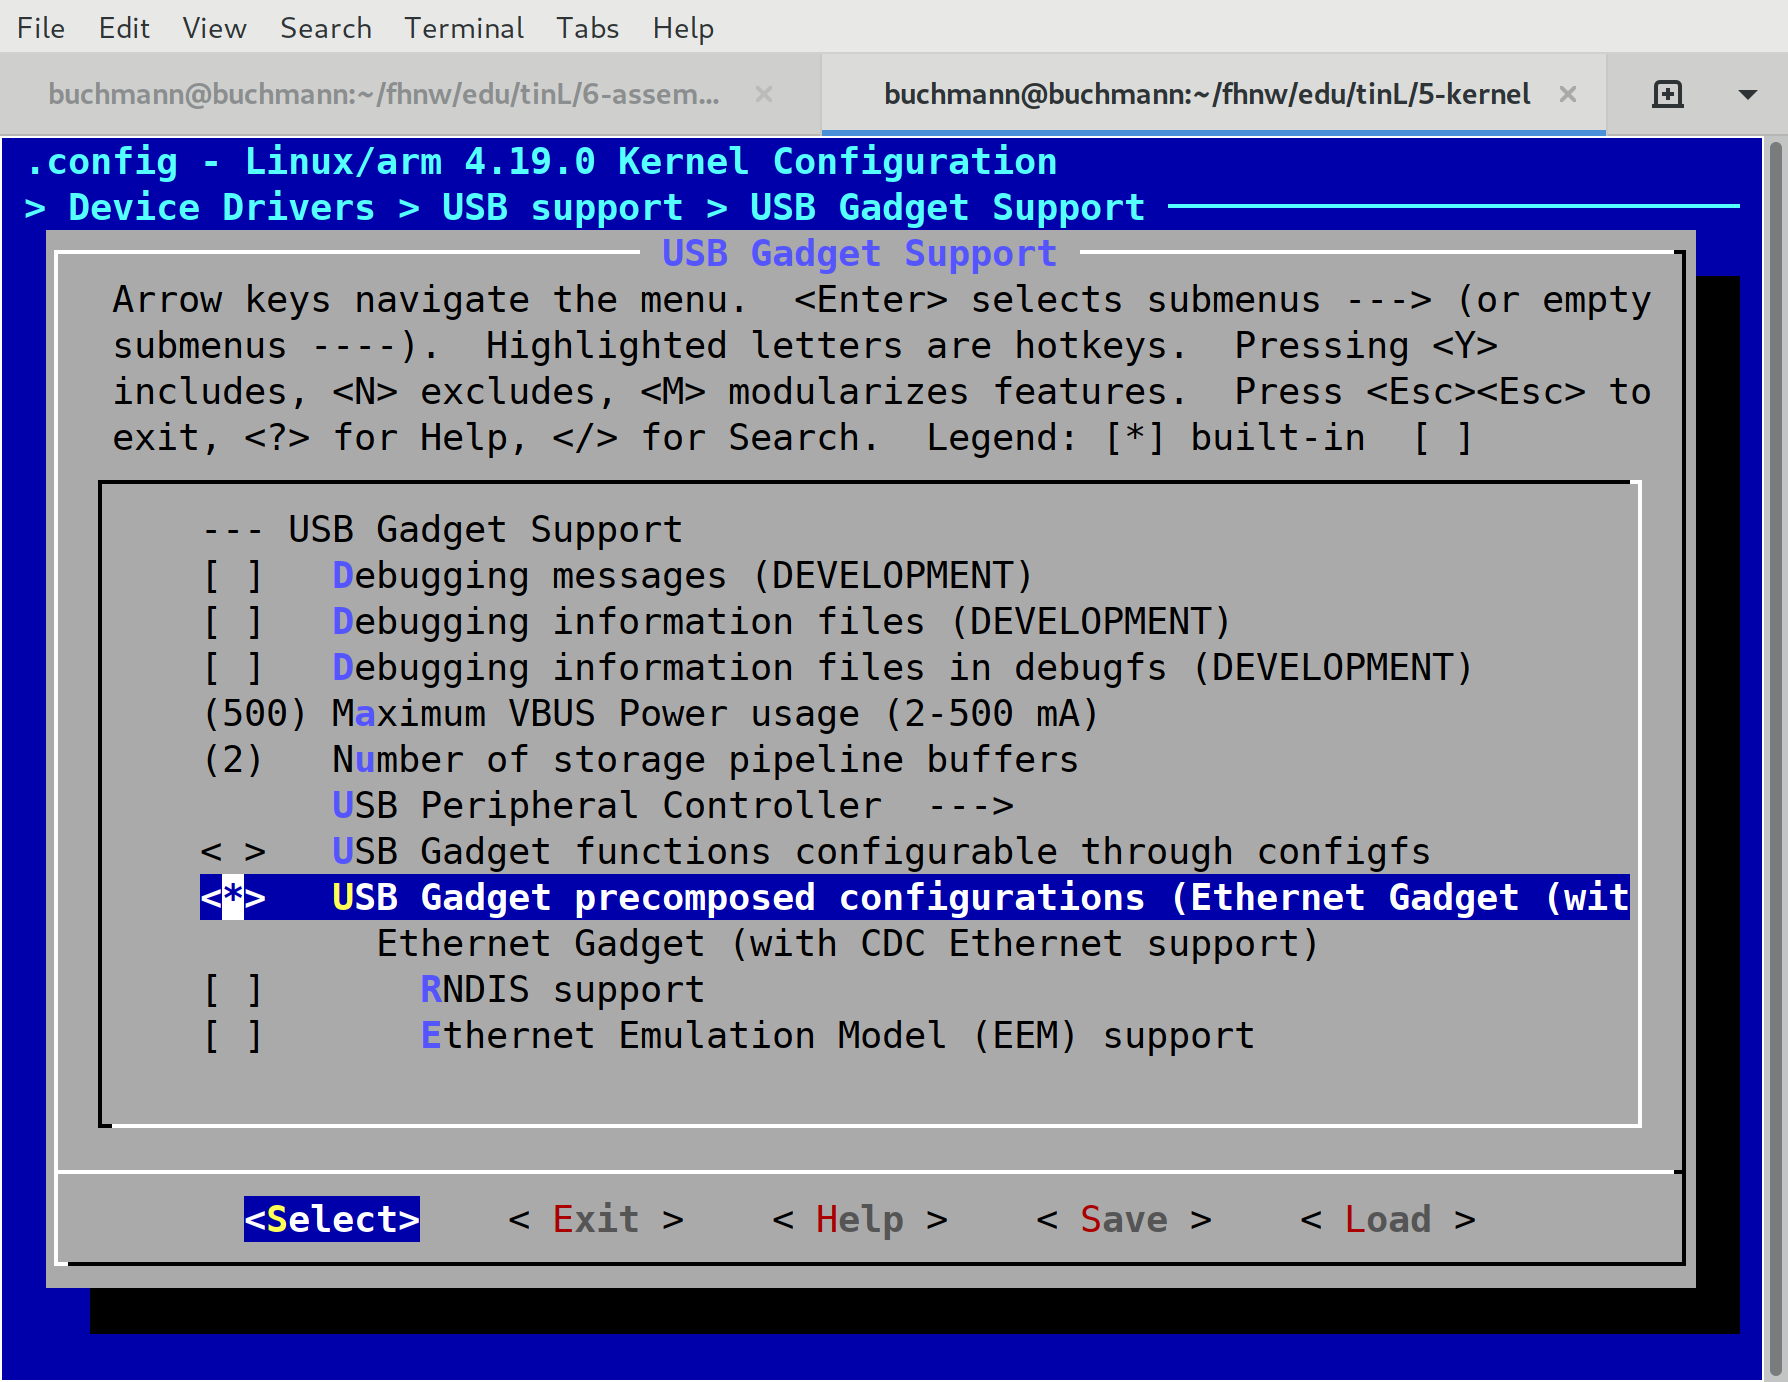
\includegraphics[height=0.875\textheight]{usb-gadget-support.png}
\end{center}
\end{frame}

\section{RootFS}
\begin{frame}{Init Script}{\cod{target-root-2016.11.22.tar.gz}}
 \begin{itemize}
  \item \cod{/etc/init.d/rcS} das {\em Init-Script}
  \item \cod{ifconfg} f�r Internet
  \item \cod{sshd} Server f�r Verbindung
 \end{itemize}
\end{frame}

\section{Aufgabe}
\begin{frame}{Aufgabe}
 \begin{description}
  \item[\uboot] Automatisches booten: \cod{uEnv.txt}
  \item[\kernel] Ethernet �ber USB
  \item[\unix] Automatisches starten: \cod{/etc/init.d/tcS}
  \begin{itemize}
   \item Internet:\cod{ifconfig}
   \item ssh Server: \cod{sshd}
  \end{itemize}
 \end{description}
\end{frame}


\begin{frame}{Workflow}{Notationen}
 \begin{description}[\cod{target-root-{\em V}.tar.gz}]
  \item[\cod{\em sd-card}] die Partition vom rootfs auf der SD Karte
  \item[\cod{target-root-{\em V}.tar.gz}] das heruntergeladene rootfs
  \item[\cod{\em target-root}] das rootfs von \targetS auf dem \host
 \end{description}
\end{frame}

\begin{frame}{Workflow}{schrittweise Verbesserung}
 \begin{enumerate}
  \item Initialer Download \cod{target-root-{\em V}.tar.gz}
  \item \cod{target-root}
  \begin{itemize}
   \item \cod{tar -xf target-root-{\em V}.tar.gz -C {\em target-root}}
  \end{itemize} 
  \item Transfer auf \cod{\em sd-card}
  \begin{itemize}
   \item \cod{rsync -av {\em target-root}/ {\em sd-card}/}
   \item \cod{sync} 
  \end{itemize} 
  \item Test/Konfiguration auf dem \targetS
  \item Update auf dem \host
  \begin{itemize}
   \item \cod{rsync -av {\em sd-card}/ {\em target-root}/}
  \end{itemize} 
  \item $\to$ 4
 \end{enumerate}
\end{frame}

\begin{frame}{Die Files}
 \begin{block}{Partition 1: vfat}
  \begin{itemize}
   \item \cod{MLO}
   \item \cod{u-boot.img}
   \item \cod{zImage}
   \item \cod{am335x-boneblack-wireless.dtb}
  \end{itemize}
 \end{block}
% \vspace{-4mm}
 \begin{block}{Partition 1: ext4}
  \begin{itemize}
   \item rootfs auf dem \host
   \item \cod{rsync -av target-root/ {\em sd-card/}}
   \item \cod{sync}
  \end{itemize}
 \end{block}
 
\end{frame}

\end{document}
